
% ********** Chapter 7 **********
\chapter{Web Application}
\label{sec:WebApplication}

\section{Overview}
\label{sec:WebApplication:Overview}

\begin{figure}[!hbtp]
\centering
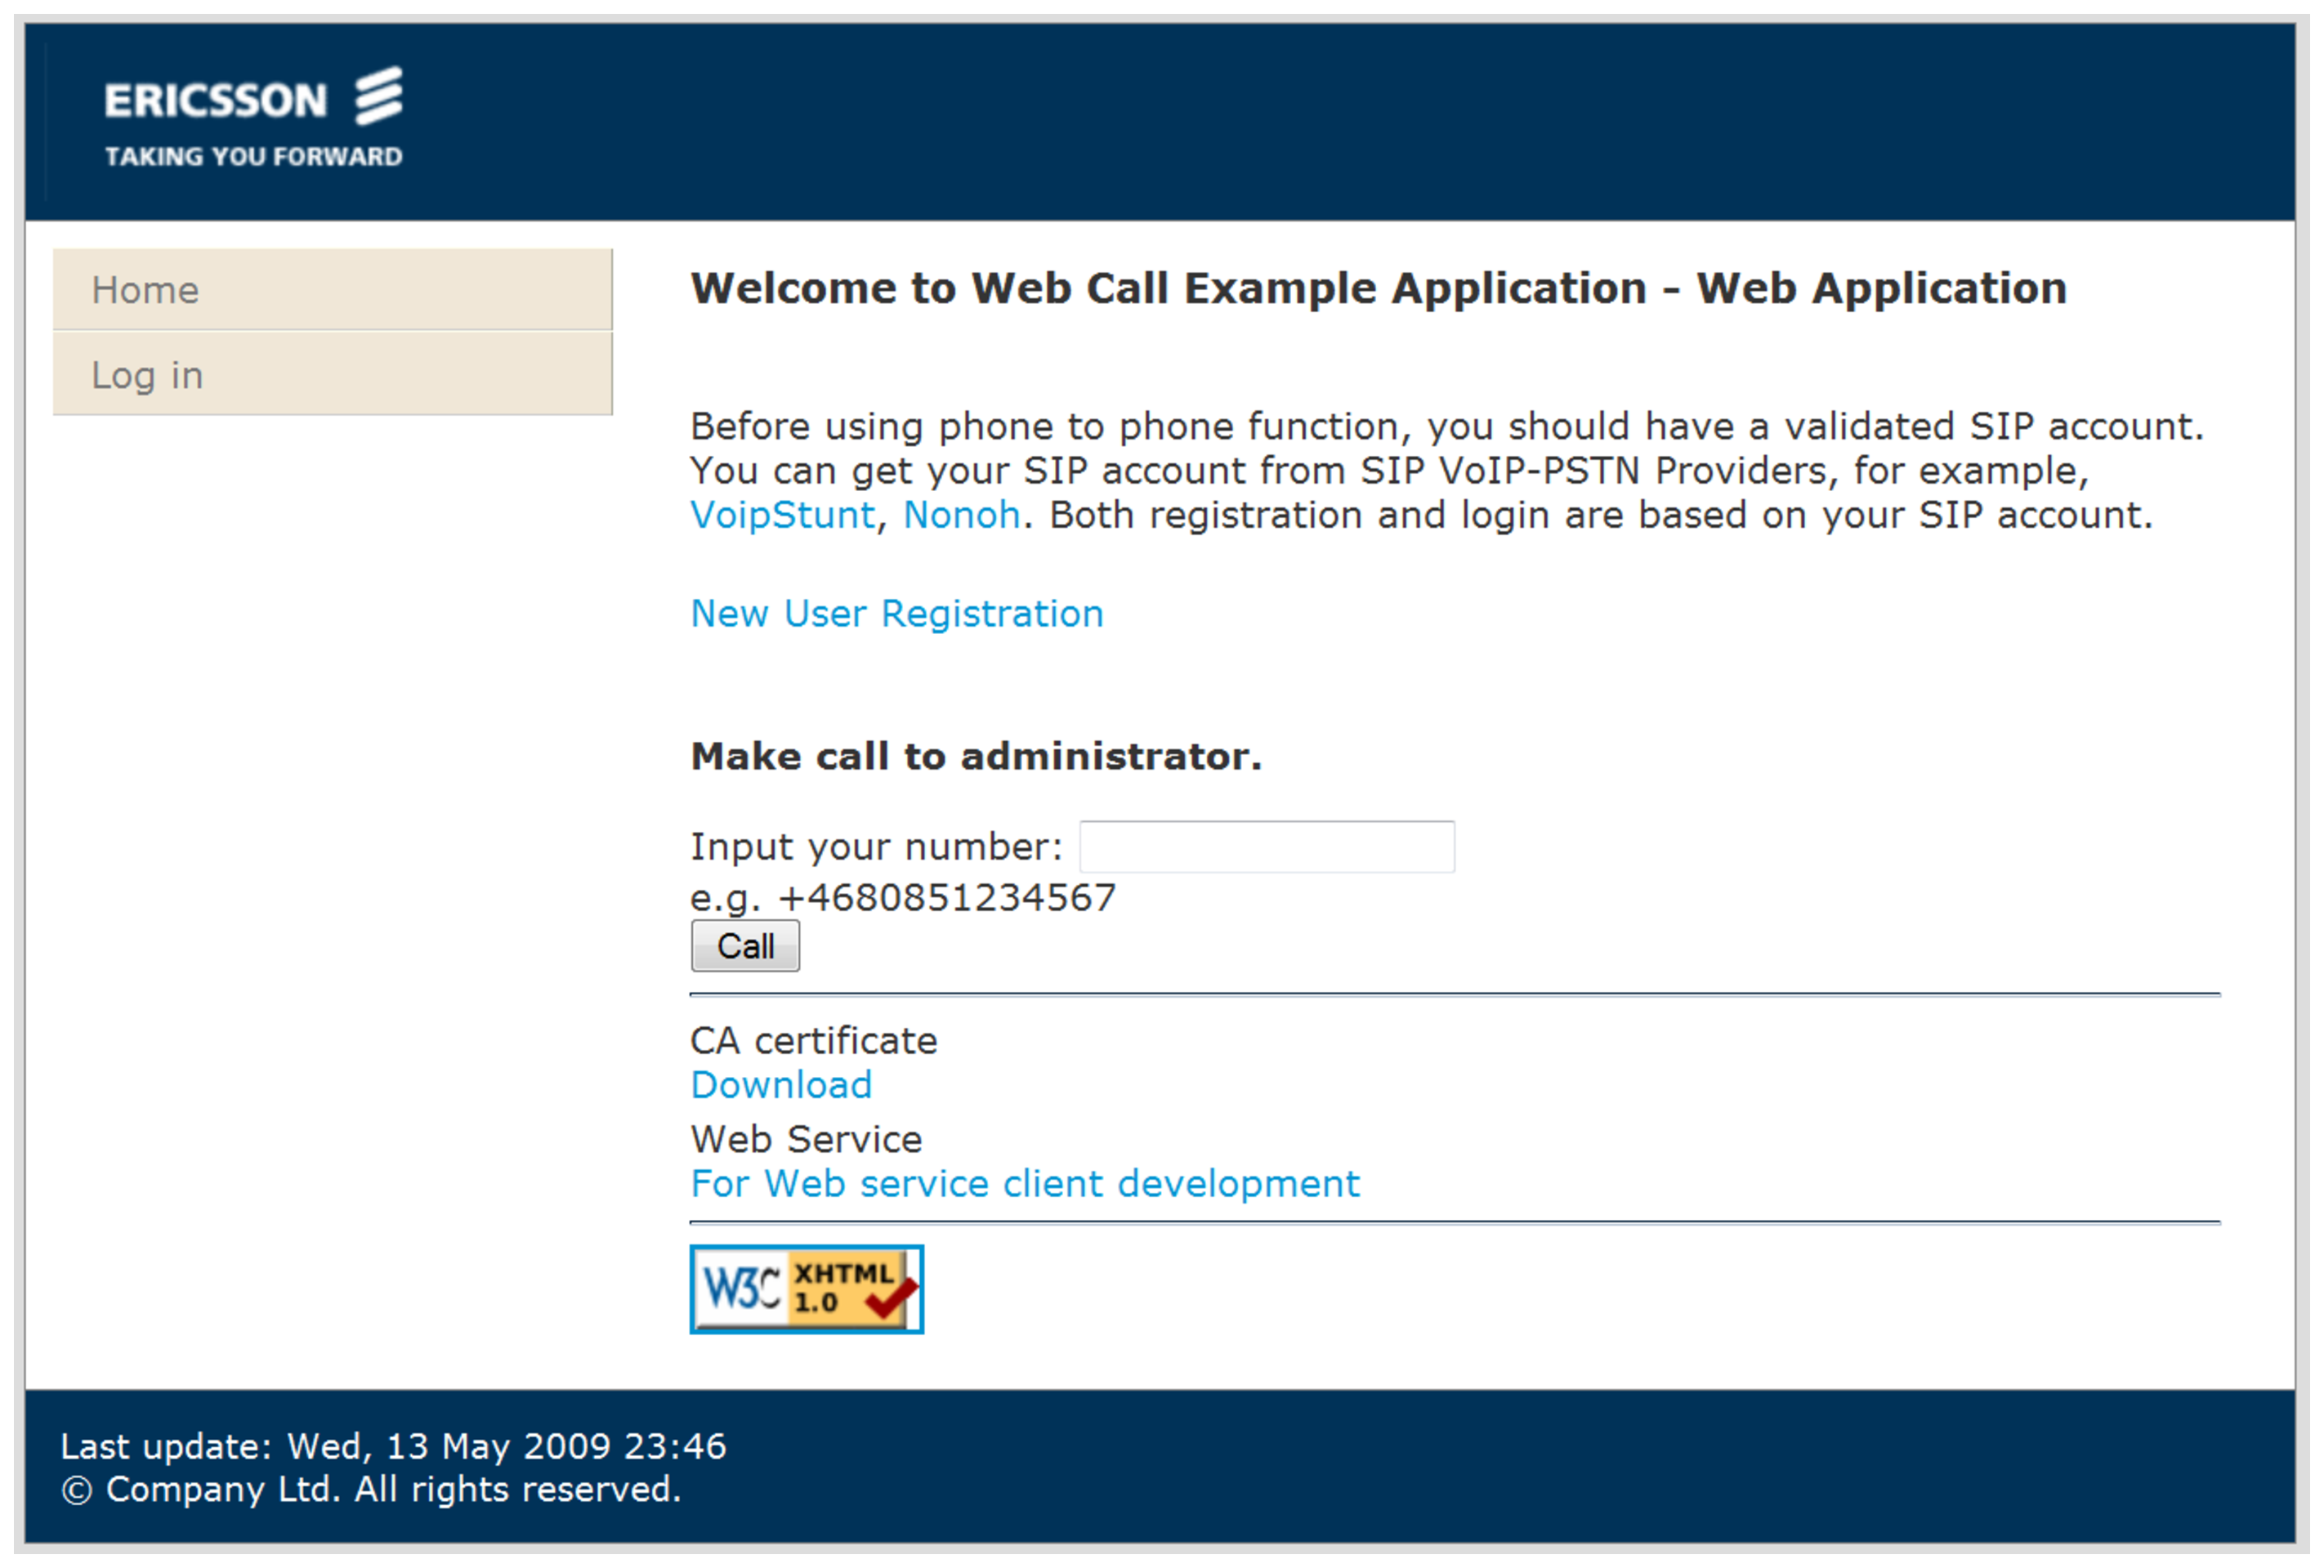
\epsfig{file=chap07/resources/welcome_desktop_browser_view, width=5.2in}
\caption{Welcome page of desktop browser view of web application}
\label{fig:WelcomePageOfDesktopBrowserView}
\end{figure}

The web application is the main portal of the whole application. It is based on Mobile Front Controller. The role of web application in the whole application is shown in Figure \ref{fig:ArchitectureOfWebCallSDK}. Users can use the web application to manage their accounts and VoIP calls. Administrators can use web applications to manage users. The web application can be packaged into a war file and easily to deploy. It only needs a sevlet container, like Tomcat, to run. It supplies two kind of views one is for desktop browser and another is for mobile browser. Beside these two views, the web application also contains a web service interface. This chapter will focus on two browser view. The web service interface will be introduced with detail in chapter \ref{sec:WebServiceInterface}.

A welcome screen of desktop browser view of Web Application is shown in Figure \ref{fig:WelcomePageOfDesktopBrowserView}.

\section{Architecture of Mobile Front Controller 3}
\label{sec:WebApplication:ArchitectureOfMobileFrontController3}

\textit{``Mobile Front Controller (MFC)\label{sym:MFC} is a light-weight Java EE web application framework for creating web applications for web browsing and mobile browsing.''}\cite{MobileFrontController} It was developed by Peter Yeung and P\"{a}r Johansson from \href{http://www.ericsson.com/developer/}{Ericsson Developer Connection}, Ericsson\cite{MobileFrontController}. The mobile front controller uses a sevlet to handle http request, and redirect request to different kind of view. All views share a same logic. An overview of Mobile Front Controller used by a web application on a Java EE web container is shown in Figure \ref{fig:MFCOverview}.

\begin{figure}[!hbtp]
\centering
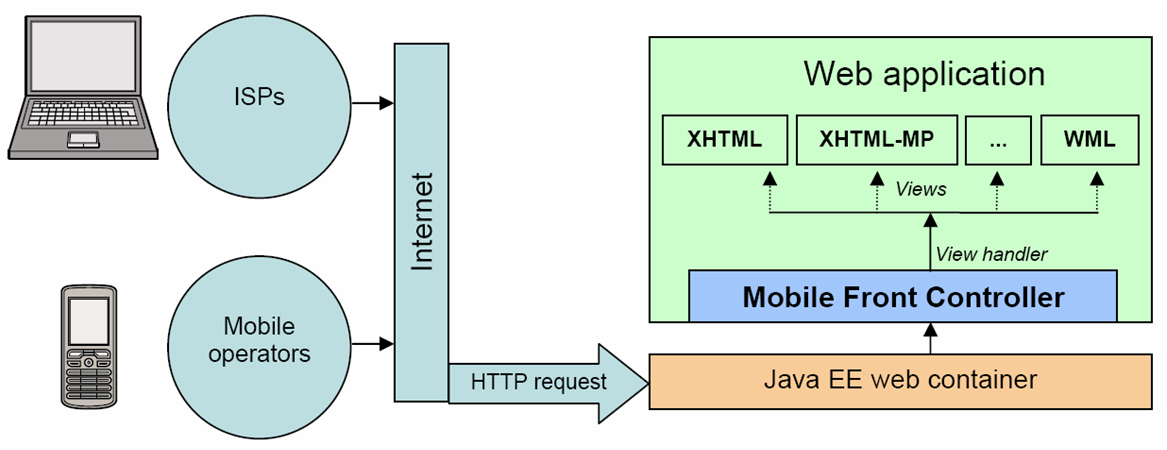
\epsfig{file=chap07/resources/MFC_overview, width=5.2in}
\caption{An overview of Mobile Front Controller used by a web application on a
Java EE web container. (Figure taken from \textit{Mobile Front Controller Developer's guide for software version 3.1}\cite{DevelopersGuideOfMFC})}
\label{fig:MFCOverview}
\end{figure} 

\textit{``MFC is used on top of a Java EE web container, and does not require any other framework, such as JSF, Struts, etc.
MFC does the following:}
\begin{itemize}
\item \textit{{Detects and selects appropriate views based on HTTP request headers. A view is a subdirectory that, for example, corresponds to a markup language such as XHTML, XHTML Mobile Profile (MP) and WML (see Figure \ref{fig:ArchitecureOfMFC}). The way MFC detects and selects views is customizable using view handlers.} }
\item \textit{Shares UI logic between different views, for example, web and mobile browsing. This is done using action commands, which are classes that contain an execute method that is executed when a URL with, for example, the URL pattern *.do is called (for example http://localhost:8080/mfc-basic-demo/xhtml/Print.do).''}\cite{DevelopersGuideOfMFC}
\end{itemize}

\begin{figure}[!hbtp]
\centering
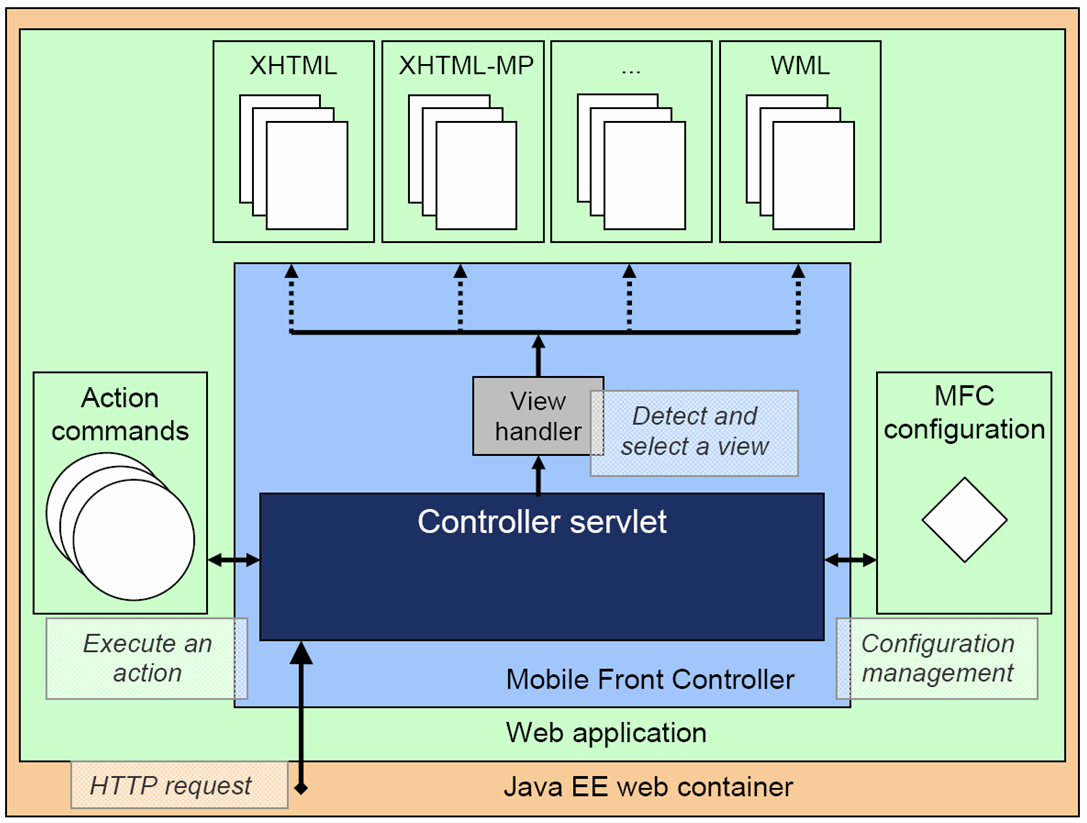
\epsfig{file=chap07/resources/architecture_of_mfc, width=5.2in}
\caption{The architecture of Mobile Front Controller (Figure taken from \textit{Mobile Front Controller Developer's guide for software version 3.1}\cite{DevelopersGuideOfMFC})}
\label{fig:ArchitecureOfMFC}
\end{figure} 

The version of Mobile Front Controller used in Web Call Example Application is the latest version, v3.1.

\section{Dual view}
\label{sec:WebApplication:DualView}

As described in the section \ref{sec:WebApplication:ArchitectureOfMobileFrontController3}, Mobile Front Controller supplies multi-view function. Web Call Example Application is developed with two view, one is desktop browser view and the other is mobile browser view. The will be illustrated separately in subsection \ref{sec:WebApplication:DualView:DesktopBrowserView} and \ref{sec:WebApplication:DualView:MobileBrowserView}.

\subsection{Desktop browser view}
\label{sec:WebApplication:DualView:DesktopBrowserView}

The Mobile Front Controller supplies a function of select view. If the user access web application via a desktop browser, the desktop browser view (XHTML view) will return to user. The desktop browser view is a normal web site that follows the standard of The XHTML 1.0. Extensible HyperText Markup Language (XHTML\label{sym:XHTML}) is a markup language for web pages which developed by W3C HTML Working Group. It is widely used as a standard language of web page on Internet. A example page (the user profile information page) of desktop browser view is shown in Figure \ref{fig:UserProfileInformationDesktopView}.

\begin{figure}[!hbtp]
\centering
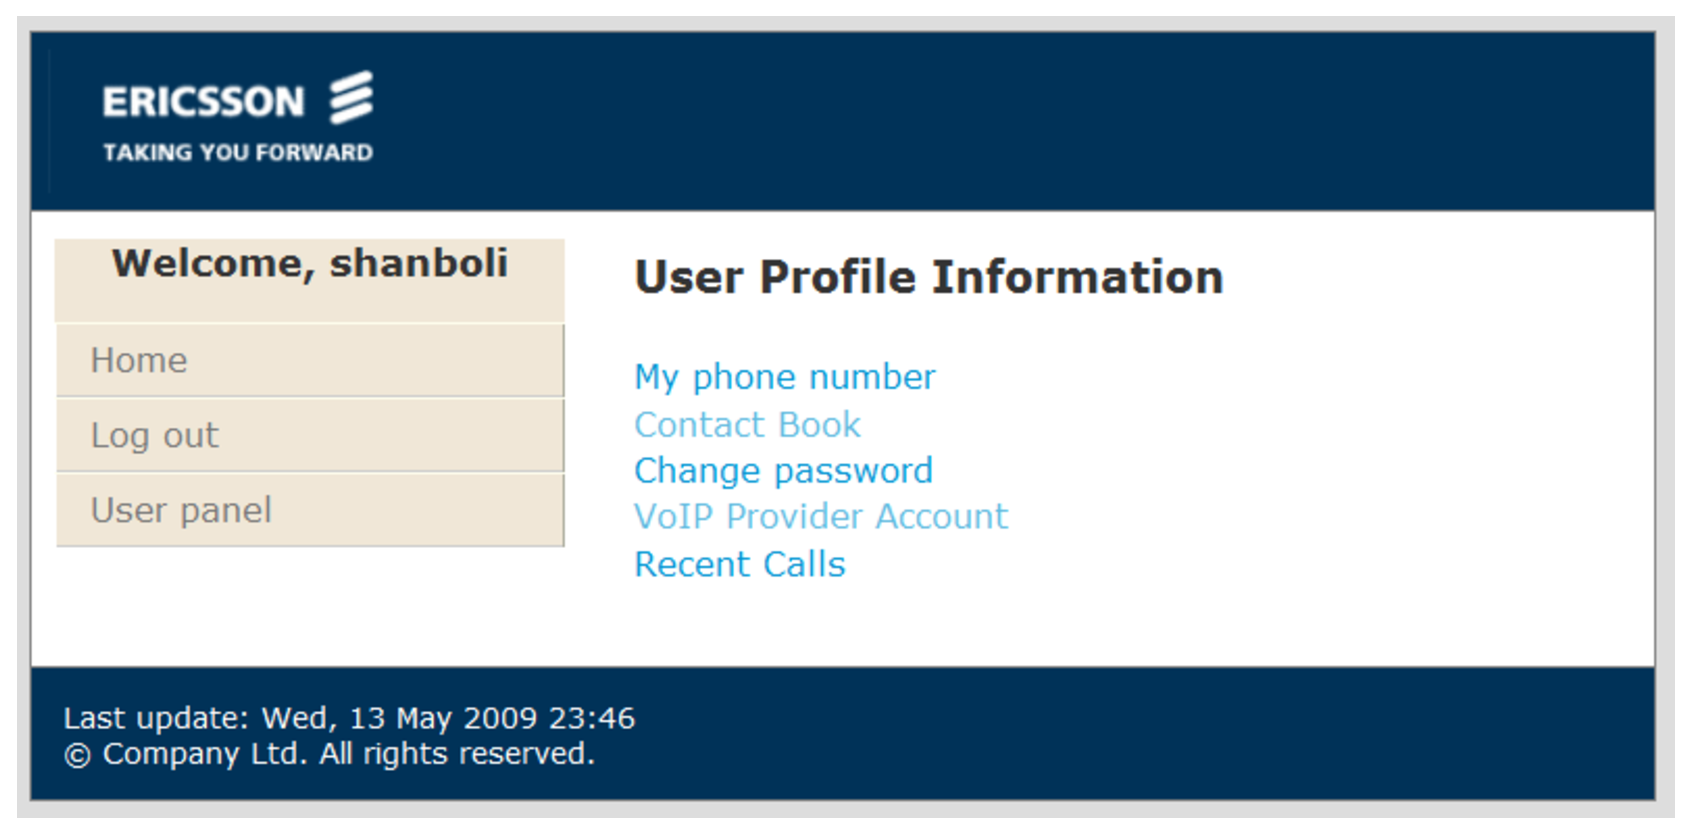
\epsfig{file=chap07/resources/user_profile_info_desktop_view, width=5.2in}
\caption{User profile information page of desktop browser view}
\label{fig:UserProfileInformationDesktopView}
\end{figure} 

\subsection{Mobile browser view}
\label{sec:WebApplication:DualView:MobileBrowserView}

If the user access web application via a mobile browser, the mobile browser view (XHTML MP view) will return to user. The mobile browser view is a normal web site that follows the standard of XHTML MP 1.1. XHTML Mobile Profile (XHTML MP) is a computer language standard designed specifically for mobile phones. It is developed by  A example page (the user profile information page) of is shown in Figure \ref{fig:UserProfileInformationMobileView}.

\begin{figure}[!hbtp]
\centering
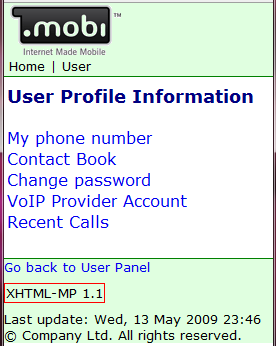
\epsfig{file=chap07/resources/user_profile_info_mobile_view, width=2.5in}
\caption{User profile information page of desktop browser view}
\label{fig:UserProfileInformationMobileView}
\end{figure} 

\section{Site structure}
\label{sec:WebApplication:SiteStructure}

The web set structure contains three levels. \texttt{Base} \textrightarrow{} \texttt{Protected} \textrightarrow{} \texttt{admin}. Both desktop browser view and mobile browser view use the exactly same structure. 

Under base directory, there is welcome page, user register page and login page. The pages on this level are public opened. There are no restrictions on requesting these pages. 

All pages in protected directory are authenticated resources. To visit these pages, the user has to login first. Both user and administrator can request this kind of resources. Under user panel, user can freely edit information, e.g. user phone number, contact book, change password, VoIP provider account and recent calls. Users can make VoIP calls by clicking the link of Phone to Phone Call under user panel. 
The pages under admin directory are used for managing user information. Only user who has a role of administrator can access pages under admin directory. Administrator can modify user information or even delete users. 
For more details about security, please refer section \ref{sec:WebApplication:Security:SecurityConstraint}.

\section{User action}
\label{sec:WebApplication:UserAction}


\section{Administrator action}
\label{sec:WebApplication:AdministratorAction}


\section{Validation mechanism}
\label{sec:WebApplication:ValidationMechanism}

The validation of web application is implemented both at presentation tier and logic tier. On presentation tier, all form are validated by \texttt{javascript}. The validation on presentation can save the time of communication between browser and server. 

\lstset{language=Java}
\begin{lstlisting}[frame=lines, float, caption=A floating example]]
import java.io.File;

public class SpaceChecker {
  public static void main(String[] args) {
    File[] roots = File.listRoots();

    for (int i = 0; i < roots.length; i++) {
      System.out.println(roots[i]);
      System.out.println("Free space = " + roots[i].getFreeSpace());
      System.out.println();
    }
  }
}

\end{lstlisting}

However, to prevent user disables \texttt{javascript}, there is also a validation mechanism on logic tier.  

\subsection{Page level}
\label{sec:WebApplication:ValidationMechanism:PageLevel}

\subsection{Server level}
\label{sec:WebApplication:ValidationMechanism:ServerLevel}

\section{Session control}
\label{sec:WebApplication:SessionControl}

\section{Ajax in web application}
\label{sec:WebApplication:AjaxInWebApplication}

\section{Java ME helper}
\label{sec:WebApplication:JavaMEHelper}

\section{Database}
\label{sec:WebApplication:Database}

\textsf{TODO: remember to write the first user will be administrator.}


\subsection{Design of database}
\label{sec:WebApplication:Database:DesignOfDatabase}

\subsection{User database utility}
\label{sec:WebApplication:Database:UserDatabaseUtility}

\section{Security}
\label{sec:WebApplication:Security}

\subsection{Certificate}
\label{sec:WebApplication:Security:Certificate}

\subsection{Security constraint}
\label{sec:WebApplication:Security:SecurityConstraint}

\subsection{Authorization}
\label{sec:WebApplication:Authorization}

% ********** End of chapter **********
